% !TEX root = ../../book.tex
\chapter{The Technology Stack\label{chap:ch_tech}}

There is a broad range of trading infrastructures and operations depending on the size and trading needs. None, however,  is as broad and complex as a low touch trading operation of a large Broker-Dealer. For this reason we use that as a template for our exploration of the technology stack necessary to support such an operation. We start by reviewing the end to end flow of information and provide some detail on various components. As previously discussed all large Electronic Trading (ET) businesses also operate their own Alternative Trading System (ATS) so we will  look at the technology setup needed to support that use case as well.



% From client Instruction to Trade Reconciliation
\section{From Client Instruction to Trade Reconciliation}

Figure~\ref{fig:TradingInfraGraph} shows the end to end diagram of a hypothetical trading infrastructure. We can use this diagram to follow the full life cycle of a client order and the main components of the infrastructure involved. \twomedskip

	\begin{figure}[!ht]
	\centering
	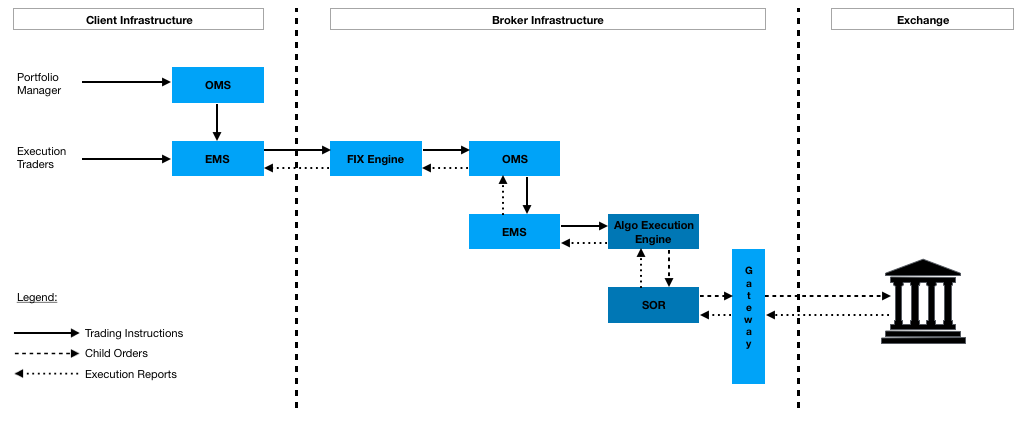
\includegraphics[width=\textwidth]{chapters/chapter_tech/figures/TradingInfraGraph.png} 
	\caption{Sample End-to-End Trading Infrastructure. \label{fig:TradingInfraGraph}}
	\end{figure}


\noindent\textbf{Client Side:} The trader enters an algorithmic order into the Execution Management System (EMS), a specialized trading infrastructure that integrates the internal systems and provides tools for institutional traders to manage day to day trading needs. EMS most often refer to vendor products, Ez Castle\footnote{\url{https://www.ezesoft.com/}}, Portware\footnote{\url{http://www.portware.com/}} and FlexTrade,\footnote{\url{https://flextrade.com/}} are some of the most popular options. Many large buy-side trade organizations have more complex needs and often seek a more homegrown solution.


The trader normally selects from a drop-down menu, a particular provider and an Algo strategy and  chooses the desired parameters. Brokers who want to expose their execution into an EMS need to certify with the EMS by providing a Financial Information eXchange (FIX) Specification document that highlights what strategies are available and what parameters are associated with each strategy and the validation information about the parameters. The EMS then integrates this into their system and exposes them in the front end for the trader to chose. FIX is a standard communication protocol specifically designed for financial applications.\footnote{\url{https://www.fixtrading.org/}} Once the order is submitted, the EMS uses a preconfigured network connection to transfer the order to the broker. This session is created as part of the \emph{Client Onboarding} step, a quite laborious process to set up a new client relationship and configure their financial limits and controls, billing, etc. \twomedskip


\noindent\textbf{Inbound Gateway:} We are now on the broker-side where the order is received by an inbound network gateway. First, it is ensured that the message is a valid order and has all the necessary fields. Next, it will perform a set of risk and credit checks to ensure that the order is within the specified risk limits and the client's overall exposure, the maximum notional the client is allowed to trade and have in the market at any point in time. If any mismatch in these validation steps is detected the order is rejected and sent back to the client. \twomedskip


\noindent\textbf{Order Management System and Order Enrichment:} Once the order is validated, the order is created within the broker dealer infrastructure. The order life-cycle is quite complicated and more nuanced. It is critical that the state of the order is always up to date and transitions in states are to be carefully managed. The role of creating and managing the state of the order is fulfilled by an Order Management System (OMS). These infrastructures are at the heart of any trading operation and they are often built around a bus-based architecture, a software paradigm where loosely coupled components communicate with each other over a messaging middle-ware. The advantage of this approach is that other ancillary components within the infrastructure can ``Listen in'' on the messages and use the information to transmit to other systems or collect data for trade reporting and analysis.


One step often performed in this layer is Order Enrichment. This is a step that adds additional, lower level parameters that adjust and customize the execution behavior for the specific client/algorithm/parameters triplet. This step also translates slight differences between the instructions the client sent and how the local execution system understands (e.g., Algo name could be sent as ``Vwap'' but needs to be ``VWAP''). This is often accomplished by a specialized \emph{Rules Engine} a software library that allows a set of rules to be applied to a structure. The rules are then reevaluated after any modification until no additional rules are triggered. \twomedskip


\noindent\textbf{Execution Strategy Stack:} As the famous quote goes: ``Is where the magic happens!'' The order reaches the software component where the Algo is actually executed. We delve into more details on the execution stack in the next section. So here, we assume that the strategy is initialized and starts executing. The strategy associated with the order contained in the OMS is often called the ``Parent Order" and as consequence of the strategy logic one or more ``child'' orders  are created in the OMS and sent forward for submission to one or more trading venues. Before the order is actually forwarded, it passes through an additional control layer, that ensures the strategy does not violate the risk limits and other ``speed bumps'', a general term used for limits that prevent the strategy from trading too fast or too aggressively or from sending too many child orders, etc. \twomedskip


\noindent\textbf{Outbound Gateway:} The child orders are received by another piece of infrastructure that is responsible for actually transmitting the orders to the market: the Outbound Gateway. All venues support additional protocols to communicate with market participants. Essentially all of them support a FIX protocol, but in most cases they also support a much faster ``native'' protocol that encodes the instructions in a compressed binary protocol. The role of the Outbound Gateway is to connect to the various venues and then act as a translation layer from the internal representation in the OMS to the external representation of the specific protocol implemented by the venue. The outbound gateway also listens in to the connection callback to capture the asynchronous events coming from the venue, like order insert/cancellation acknowledgments and executions and in turn updates the state of the child order representation in the OMS. \twomedskip


\noindent\textbf{Notifications to the Client:} As the strategy executes orders in the market, the OMS keeps the state of the parent order up to date with each execution and sends periodic updates via the inbound gateway back to the client's EMS that updates its own state and provides feedback to the trader that the strategy is executing, the average prices currently achieved, and other analytics necessary for the trader to understand how well the strategy is executing. The inbound control layer is also kept up to date so that the total state of all client orders is accounted for if and when a new order from the same client is received. \twomedskip


\noindent\textbf{Middle and Back Office:} We are now almost done. The step above completes the real-time feedback loop from the client through the executing strategy to the market and back. The rest of the processing is in most cases done offline by a set of infrastructures commonly referred as ``Middle and Back Office Systems''. These systems play a critical role in the business and regulatory side of trading. They are arguably the most important piece of the puzzle, without which no trading operation could function. As we previously discussed, performance of an algorithm is really just the cherry on the trading cake. Without a trader knowing what has been traded and what their current positions are, without the confidence that a once a buy order is executed, within the $T+2$ settlement period (more on this below) the shares the trader just bought will be in the trader's account, nothing else would matter. Describing in detail the complexity and subtleties of the process that ensures that once an order is executed, the shares or the monies are in the right account at the right time is well beyond the scope of this book. But the authors feel it is important that the reader has at least some understanding and a high degree of respect for the critical role these systems. The hard working people who operate them often spend nights and weekends handling the myriad of exceptions and trade breaks that are unfortunately all too common in the industry.


To start, let us quickly review the process by which share ownership is transferred between large institutional sellers and the buyers. Stock ownership is almost never in paper form but is very likely stored as a book entry in a computer at a place called Depository Trust Company (DTC). This firm acts as the main custodian for all the shares that can be freely traded on an exchange. Brokers will have an account at the DTC that keeps custody of all the shares the broker holds on behalf of their clients. From the DTC perspective the broker is the owner of the shares. The process of transferring ownership goes through two steps:
        \begin{itemize}
        \item Clearing: It is the process of updating the accounts of the trading parties and arranging for the transfer of money and securities. In most cases, this step goes through yet another intermediary, a Central Clearing entity that provides various services; in particular, all trade aggregations so only the net shares across all trades are  transferred.
        \item Settlement: It is the process of actual exchange of securities for cash. This in most cases (there are always exceptions in a complicated process) happens at $T+2$.
        \end{itemize}
The DTC then also handles other functions like the handling of all stock dividends and other corporate actions.


As discussed previously, in general, investors cannot trade directly with each other but  only through an intermediary, a Broker. Many investment institutions often trade with multiple brokers but engage one (and sometimes more than one) as a Prime Broker where they centralize their balances. Prime brokers provide all set of services, e.g. stock lending, financing, etc. The client will set up one or many accounts with the prime broker (sometimes thousands, depending on the complexity of the operations) where they record, which shares registered in DTC, do actually belong to the client. Some of the largest and most complex institutions, to limit credit exposure and for other competitive reasons, leverage multiple Prime Broker relationships in an even more complex Multi-Prime setup. 


Let us finally turn to the main topic. In executing, broker middle and back office operations are segregated into two distinct parts and are managed independently: 
        \begin{itemize}
        \item The Market Side: This deals with the interaction with the various exchanges  and the clearing house and ensures that there is a perfect match between what the broker thinks, what has been traded and what actually was traded, at what price and how, i.e. taking vs. providing. This then is used to actually determine to whom the broker needs to pay, the various exchanges for their execution fees (or get paid by them if a rebate was earned).
        \item The Client Side: This handles the clearing and allocation of all traded shares to various accounts based on the client instructions (mostly in electronic format but sometimes even via email!) and ensures that their records match exactly with both the clients and the prime brokers. It also handles all reconciliation of the all too frequent ``trade breaks'' when something does not quite matche exactly.
        \end{itemize}


The two sides (Market and Client ) are usually separated in a set of Middle office functions that handles the booking and allocations and the confirms with the client/exchanges and a back office that manages issues around settlement. The back office also handles the regulatory burden of  managing the trade reporting process to the TRF/ACT and the OATS process that sends to FINRA, the full life-cycle of the order. As the reader can now appreciate, the role of this function that is absolutely critical to the correct functioning of a trading operation. The middle and back-office teams are truly the unsung heroes of this endeavor. Without them, what we do would not matter one single bit.



% Algorithmic Trading Infrastructure
\section{Algorithmic Trading Infrastructure}

This section details a somewhat generic approach for algorithmic trading infrastructure. Different providers have different approaches to this. For instance in some platforms, the core strategy is in one infrastructure but the order routing part is a separate (albeit similar) infrastructure. Others combine the two together, while some separate scheduling and order placement/routing components. The simplified discussion below assumes an all-in-one approach.

	\begin{figure}[!ht]
	\centering
	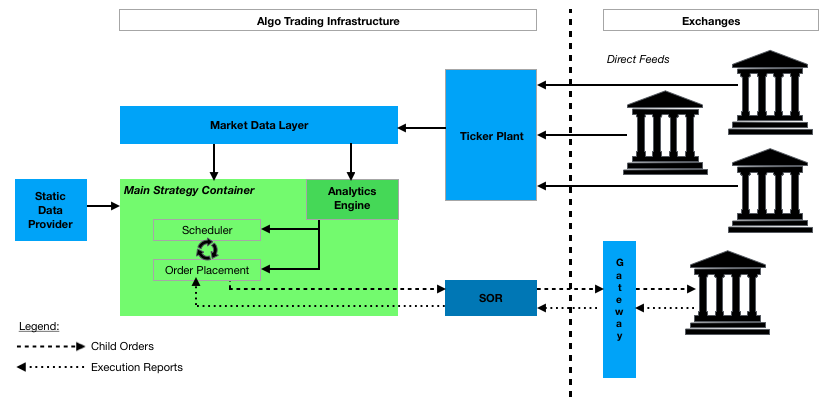
\includegraphics[width=\textwidth]{chapters/chapter_tech/figures/AlgoInfraGraph.png} 
	\caption{Sample Algo Trading Infrastructure. \label{fig:AlgoInfraGraph}}
	\end{figure}
	
The core of an Algorithmic Trader infrastructure is a software framework generically called ``Strategy Container.'' This facility sits in-between the low level OMS related functionality and the strategy and provides a set of abstractions and interfaces to simplify the development of a trading algorithm. When a new order event is received from the OMS, the strategy container reads and validates the instructions like the name of the strategy and the necessary and additional parameters. If this is a valid new order instruction, it usually has to pass through an additional layer of controls to ensure that other variables such as order quantity or limit price are within the required boundaries. Once this validation step is completed the strategy container instantiates the code of a particular strategy, initializes it with the specific parameters. It will also connect the algorithm to the necessary services that the algorithm needs for implementing the strategy. Let us look at some of the main services and related infrastructures. \twomedskip


\noindent\textbf{Static Data Services:} An Algorithmic strategy requires a non trivial amount of reference data and other static data to operate. First and foremost, the particular instrument the strategy is trading but also other information like what the primary exchange is, open/close time of the exchanges, etc.. It will also require the normalizing analytics as well as any calibration parameters for various models. These static data services abstract the sources of the underlying data that could be databases, flat files and provide calls to other systems. \twomedskip


\noindent\textbf{Market Data Facility:} Access to real-time market data is the most important component of any trading algorithm. Strategy container is usually provided with two ways of accessing this data: via a data cache that is continuously kept up-to-date by an underlying thread, and via callback. The data cache also continuously updates additional core analytics used by the strategy such as total traded volume (filtered for specific condition codes) and others. A natural question is how do we actually get real-time market data? Connected to our market data facility is one of the most demanding and expensive pieces of infrastructure in the whole stack: the Market Data Plant. This is worth a small detour for a brief discussion. \twomedskip


\noindent\textbf{Market Data Plant:}  Any serious trading operation, in particular in the post NMS and OPRS era requires to access protected quotes, to subscribe and deliver direct market feeds from all registered (thus protected) exchanges. For most use cases, top of book (Level~I) data is not going to be sufficient. It is necessary to subscribe to at least Level~II or even better Level~III data. Each exchange family (and sometimes even within one) has its own proprietary multicast protocol. Also very important information like trade condition codes are also proprietary and are to be normalized. For each Level~III market data feed, a book building library is needed that interprets all the multicast events and updates the internal state of the book. Doing this in a very efficient way that can withstand market data spikes without dropping any multicast packet is not an easy task. It requires skill and an excellent networking and computer infrastructure, something that is quite expensive to build and maintain. For this reason trading operations often rely on third party vendors for this component that can provide a hybrid software and hardware solution to handle the entire operation. Some of the vendors in this space are: Reuters,\footnote{\url{https://financial.thomsonreuters.com/en.html}} Redline Trading Solutions,\footnote{\url{https://www.redlinetrading.com/}} and Exegy.\footnote{\url{https://www.exegy.com/}} Over and above the hefty cost of operations, exchanges have in the last decade significantly increased the cost of subscription for market data. This is now a significant component of the overall cost of running a trading operation (in the seven digit range!). \twomedskip


\noindent\textbf{Outbound Order Interface:} Now back to the discussion of the core services. The last core set of abstractions has to do with managing outbound child orders. This facility provides the strategy with the state of all outstanding child orders and ability to create, cancel and amend them in an asynchronous way and manage any exceptions like for example, canceling an order that has just been executed on exchange but the fill event has not yet reached the OMS. \twomedskip


\noindent\textbf{Main Strategy Loop:} 


We come to the \emph{core of the core} of the whole infrastructure. While there are many ways to write a trading strategy a pattern has emerged over the years that can be described as somewhat as a standard approach. It is sometimes referred to as the Main Strategy Loop,\footnote{Some practitioners for example believe that the right conceptual framework for a strategy is that of a State Machine: Based on what event just happen there is a ``state transition'' in the next state and writing a strategy is essentially to model and implement these state transitions. Conceptually elegant, in practice this approach is extremely hard to pull off as there are a lot of side effects and co-dependencies that makes it hard to cleanly decompose.} as described in Figure~\ref{fig:MainLoop}. 

	\begin{figure}[!ht]
	\centering
	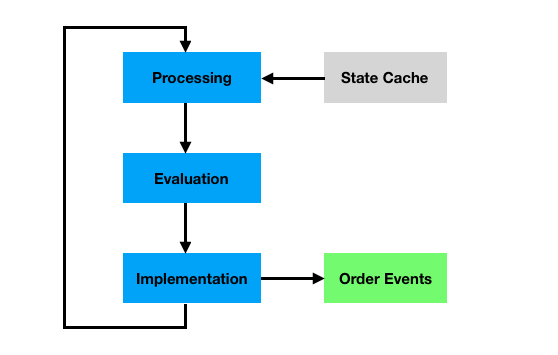
\includegraphics[width=\textwidth]{chapters/chapter_tech/figures/MainLoop.png} 
	\caption{Sample Main Strategy Loop. \label{fig:MainLoop}}
	\end{figure}
	
While the strategy container interacts with other working threads, and ensures that the state is always kept up to date, the core of the strategy flow is encoded in one stateless function. This function is called on either by a timer, any major event such as quote change/trade/execution, etc., or even on a tight loop. It  then sequentially executes three separate stages:
        \begin{enumerate}
        \item\emph{Processing:} Understand where the strategy is at any point in time by recovering the state from the state cache with all the information it needs. How many shares have been traded, and how many, based on the target strategy, should be traded and where should the traders stand in the near future. 
        \item\emph{Evaluation:} Based on the full information set and the current state of the outstanding child orders in the market, determine which orders to cancel, which to amend, and which to submit.
        \item\emph{Implementation:} Send these instructions to the Outbound Order Interface. In some cases Step 2 just calculates the correct exposure it wants in the market and it is the role of the implementation step to optimally decide if and how this should be implemented: either by submitting additional orders or by amending the existing ones, etc.
        \end{enumerate}
After performing these three steps, the main loop will exit and repeat at some time in the future. Since the approach is Markovian, meaning only the existing state matters; if the strategy is called again immediately after, it will most likely make the same decisions it just made and determine in Step 2 that no action is necessary. Thus, the main loop simply exits. \twomedskip


\noindent\textbf{Additional Infrastructures:} Depending on the complexity and sophistication of the operation, the technology stack is often supplemented by additional components that serve certain specific roles. Let us look at some of the common ones. \twomedskip


\noindent\textbf{Realtime Analytics Engine:} More and more, algorithmic trading products have become highly sophisticated and dynamic and adapt as market conditions change. The normalization variables and signals are adjusted at every single tick or after every few trades to provide the most up-to-date picture of the immediate past and future market state. Conceptually these analytics could be built within the actual strategy engine but it is not only more cumbersome, it is also inefficient. In most cases one process cannot handle the computing load to run thousands of algorithms on all symbols. The infrastructure is thus ``striped'' in multiple processes handling a subset of symbols. Per symbol analytics could still be built within each process but many analytics, like for example computing the real-time price of an index midpoint, requires that the data on hundreds or thousands of symbols to be computed in the same process. For each symbol, this would create large duplication, reducing the effectiveness of striping. Additionally with more analytics, more load on the process is created that is used to handle the algorithmic decisions.


For these and other reasons of convenience needed in calculating real-time analytics, it is often delegated to a dedicated infrastructure. This makes it easier to build additional analytics and to combine existing ones with the more complex signals. \twomedskip


\noindent\textbf{Algorithm Switching Engine:} Most execution strategies have limited flexibility to change behavior in particular situations and opinionated traders may have strong beliefs that a different trading approach might be warranted in certain situations. Historically that trader may work with one of their favorite brokers to build a customized strategy for the purpose but that usually a long time and then the trader can use this approach with only one broker. 


To provide simple dynamic customization, brokers began offering Algo of Algos functionality around what is commonly called an Algo Switching Engine. This Engine is a combination of a simple strategy container and a limited real-time analytics engine, where an Algo is represented by a simple set of if-then-else rules. The condition  part of these rules will be simple combinations of the available signal and the action part will define a particular algorithm with associated parameters. Once the order is received by the switching engine the rules are evaluated and an order for the specified strategy is sent to the strategy container. The rules are then re-evaluated every few seconds and if the conditions change the switching engine will send a cancel/replace message to the strategy container to change the underlying strategy. \twomedskip


With this simple approach, one can build very sophisticated dynamic algorithms thus offering almost unlimited capabilities. This has made algorithm switching engine very popular both with traders and with execution consultants that often differentiate themselves by smart usage of the switching engine. While Algo Switching Engine is a very powerful tool, it has several meaningful downsides that one should consider:


\begin{itemize}
\item The rules that make up a custom strategy encode certain beliefs on the value of a particular triggering condition. If that condition had true predictive power it would be better integrated as an alpha signal and leveraged in a more nuanced way within the strategy rather than as a blunt instrument of an algo switching instruction. If the condition is actually, as most often the case, not predictive then the realized performance of the strategy will be, in general, made worse by the customization. Thus, while in principle, it is a good idea in practice, it should be discouraged unless its real value can be measured. This would make algorithm switching engine ideal as a temporary exploratory tool rather than the overused tool as it currently is.

\item  Algorithms are usually poor at persisting state across a cancel/replace transition. This usually implies that all state of the algorithm is lost and a completely new order is created. Algos also perform relatively poor at the beginning of the order as various analytics and execution bands exhibit poor performance when initialized (e.g. participation bands unless handled correctly have a discontinuity at zero). Frequent use of switching transitions will have severe negative impact on algorithm performance.

\item Once a trader is onboarded into a custom strategy, any Post Trade support by the broker is lost since the optionality embedded in the switching to a large extent relieves the broker from any obligation as the performance will be largely driven by the switching rules. Additionally, these orders cannot be used by brokers to measure and improve their own performance because the individual slices will be hopelessly biased by the switching rules
\end{itemize}


As one can glean from the above treatment of algorithm switching engine, the authors are not big fans of this approach and believe that this evolution has resulted in decreased quality of execution algorithms. The popularity of these approaches is still quite high and we believe currently the approach is overused. However, there are signs that this popularity is slowly waning as clients are starting to rely on the broker to fine tune the behavior of the strategies. \twomedskip


\noindent\textbf{Portfolio Algorithm Engine:} As we discussed in Chapter~\ref{chap:ch_exec_models}, some algorithmic strategies involve the coordinated trading of an entire portfolio of instruments. In this section, we briefly look at the technology infrastructure needed for these strategies and some related common issues. 


The problems start immediately, at the interaction between the FIX infrastructure and the client's EMS. Until recently Basket trading was never well supported by various EMSs making the certification of a portfolio strategy, a potentially very fiddly proposition, as it requires supporting multiple approaches. Wherever basket trading is not supported, firms have resorted to simple ways like considering every portfolio order sent to that algorithm within a certain timeframe, or linked to a portfolio ID parameter, or a combination of both.


The portfolio algorithms infrastructure is not dissimilar to the one used in Algo Switching but with the added complexity  of having to manage the schedule for multiple orders simultaneously. These algorithms will create a set of linked trajectories, often through some form of portfolio optimization process that implements the specific objective function. Once the trajectories have been generated the algorithm will, in most cases, use one or more existing algorithms possibly modified to adapt to the portfolio infrastructure.  Certain algorithm implementations send short time slices to a TWAP algorithm (essentially transforming the trajectory into a piece-wise linear curve) while other implementations may use a modified VWAP style algorithm that supports a special parameter to overwrite the trajectory to be used. Once the portfolio trading starts, market conditions changes or realized deviations of the portfolio shape (e.g., usually as an impact-control measure, the single slice will have maximum POV constraints applied, which if triggered, will distort the original intent) will often require the algorithm to re-optimize the joint schedule and the individual slices are amended to account for the changes.


This workflow is already quite complex but there are several additional mechanical and numerical issues that further complicate matters making portfolio algorithms really hard to pull off successfully. Here are some practical issues:

\begin{itemize}
\item Among the portfolio IS style algorithms, the most common optimization approach is usually implemented as a Quadratic Programming (QP)\footnote{\url{https://en.wikipedia.org/wiki/Quadratic_programming}} optimization problem where the schedule is discretized into bins representing the shares to be traded in a certain period.  For large portfolios common in fund rebalancing and for relatively fine grained time bins, the number of variables that need to be used, explodes pretty fast (in particular formulating these problems require use of several auxiliary variables to manage cost constraints, etc.). For example, a 1000 stock portfolio with 5m bins  sent to a whole day Portfolio IS algorithm would have to solve a problem with more than 100k variables. This often results in a very slow  optimization cycle that can take hundreds of seconds making it too slow for effective utilization (no client would want to wait several minutes to see the first trade!) and too intensive computationally for a scalable operation  (e.g. typically a dozen such portfolios arrive at the beginning of the day). To solve this problem effectively requires nontrivial numerical methods that make the actual optimization problem very difficult to solve.

\item Essentially, all such algorithms are discretized in time bins, and hence synchronizing the re-optimization steps to correctly line up with the executing algorithms is not easy and often leads to purely mechanical distortion of the realized schedule, even in very simple settings (e.g. the tendency of the orders to be behind schedule leads to the unexecuted quantity to be reallocated to the remaining bins causing a significantly stretched execution schedule).

\item The portfolio level optimization problem requires a variance-covariance matrix for all instruments in the portfolio. As discussed, the universe of security that are traded with algorithms is usually very large and to have stable covariance matrix for such universe requires the creation or purchase of a Factor Risk Model (either a fundamental factor model or maybe a simpler PCA style model, see Chapter~\ref{ch:amp}). New issues and ticker change create additional operational issues for these algorithms.

\item Optimization linked schedules are very rigid and to avoid significant breaches of the provided constraints, the algorithm has to follow the schedule quite closely. This means that the algorithm usually cannot leverage additional opportunistic liquidity. In a market structure like the US where 30--40\% of the liquidity is in dark pools this makes these algorithm not very effective in sourcing liquidity. Some effort in incorporating dark pools into the optimization problem was attempted in Kratz and Sch\"oneborn (2014)~\cite{kratzschon} but almost no production algorithm the authors know of have actually solved this problem effectively. 
\end{itemize}



% HFT Infrastructure
\section{HFT Infrastructure}

We have completed the whirlwind tour of the technology stack that one would find in a standard execution business. As mentioned, we did  that because it is probably the most complex and broad use case. For other setups, some of the components may be very similar, but others may differ. There are probably a dozen different configurations and discussing all of the nuances in detail is well beyond the scope of this brief chapter but as a comparison we take a quick look at the other extreme, an HFT infrastructure.


In broad terms, HFT setup is in some ways a lot simpler while others may have technical complexities beyond what are usually found in execution. To begin with, HFT strategies are not driven by instructions; thus, there is no need for all inbound connectivity, OMS, etc..  Additionally in order to achieve the maximum speed and the lowest  ``tick-to-trade'' latency,\footnote{The total time it takes from a new market data event happening on exchange (tick), to that tick being received by the trading engine which in turn generates an order, to that order reaching the exchange.} in general, the technology stack is condensed to run all in the same process. Direct market data feeds and direct exchange connectivity are just components of the same process reducing the complexities of a separate ticker plant, communication bus, and connectivity layer all together. 


If the trading operation sits outside a broker-dealer, then the trade has to go through a third party broker-dealer via a sponsored access agreement. This usually requires that the trading system will connect to a broker provided appliance or software layer and through that connect to various venues through the native market access protocols. In most cases, the trading infrastructure is co-located in the same data center as the exchange(s) where that strategy will operate.


Finally, the other main difference is the need for the infrastructure to connect to a position keeping system to incorporate the current inventory as part of the decision making. Usually these positions are also computed internally, based on start of days positions. In order to have an internal verification with additional controls, if the positions calculated internally deviate from the position calculated by the position keeping system.


What other areas then do the technical complexities that exist beyond standard infrastructures? It is often driven by the pursuit of absolute speed and throughput. This implies that it requires that having deep understanding of the networks, hardware and software, utilizing all the options in the book to squeeze additional nanoseconds. This includes specialized network switches, CPU overclocking, kernel modifications, use of assembly/machine language for the most latency sensitive parts of the codebase. It could also include setting up connectivity to far away exchanges, most notably the CME exchange where the S\&P 500 Futures is traded using proprietary networks like spread networks (now part of Zayo Group)\footnote{\url{https://www.zayo.com/private-dedicated-networks/}} or via Microwave Towers like what is provided by the ICE \footnote{\url{https://www.theice.com/market-data/connectivity-and-feeds/wireless/chicago-to-new-jersey}} and more recently also millimeter Wave Lasers like Anova\footnote{\url{https://anovanetworks.com/}}. More and more frequently, large portions of these ultra low latency setups leverage Field-Programmable Gate Array setups (FPGA)\footnote{\url{https://en.wikipedia.org/wiki/Field-programmable_gate_array}} and some vendors are even selling FPGA chips for all-in-one appliances where  feeds, connectivity and strategy are programmed in hardware.



% ATS Infrastructure
\section{ATS Infrastructure}
\subsection{Regulatory considerations}


Alternative Trading Systems (ATS), are private US\footnote{Under European regulations, ATS are designated as Multilateral Trading Facilities (MTF) and are governed by their own set of rules} securities trading platforms that meet the definition of "exchange" under federal securities laws but are exempt from registration as national securities exchange so long as they comply with the specific rules\footnote{Rules 300--304} of Regulation ATS.


Regulation ATS establishes a regulatory framework for ATS, and mandates that all ATS need to be registered as a broker-dealer with the SEC and file a Form ATS detailing the functioning of the venue and them make this documentation available to the investing public.\footnote{\url{http://www.FINRA.org/ATS}} As of January 2019, FINRA adopted an amendment to Reg ATS requiring the filing of a new Form ATS-N, addressing some of the shortcomings of the previous Form ATS, in particular around disclosure of potential conflict of interest and risks of information leakage arising from the ATS-related activities of the ATS's broker-dealer operator. The new form also discloses information pertaining to order types and market data used by the ATS, execution and priority procedures, and any process in place to segment orders in the ATS.


Three main types of venues fall under the definition of ATS:

\begin{itemize}
\item{\textbf{Electronic Communication Network (ECN):}} a computerized network allowing the trading of financial products outside traditional stock exchanges (even outside of traditional exchange hours), matching orders for a fee. As discussed in Chater~\ref{chap:ch_intro} ECNs are the historically the first setups create to compete against the monopoly of the exchange with the first ECN, Instinet, dating back all the way to 1969. 

\item{\textbf{Crossing Network:}} operated as broker-dealers' internal crossing network, matching orders in private using prices from public exchanges.

\item{\textbf{Dark Pool:}} private securities trading platform offering an undisplayed order book and matching engine. Dark pools also come in different flavors:
        \begin{itemize}
        \item{Independent dark pools:} e.g. Instinet, Posit, Blockcross, Liquidnet 
        \item{Broker-dealer dark pools:} where clients of the broker interact, such as  CrossFinder, MSPOOL, SigmaX, JPMX, LX, \dots
        \item{Hidden liquidity of public exchanges:} e.g. BATS, NYSE, ASX CenterPoint in Australia. These, however do not fall under the ATS designation per se.
        \end{itemize}
\end{itemize}


As private securities trading platforms, ATS which have an average trading volume of less than 5\% of the aggregate daily volume in NMS stocks do not need to provide a feed of their top-of-book quotes to a national securities exchange, nor are they bound by fair access rules and thus allowing them to bar access to anyone they choose.\footnote{For instance, Luminex is a pool only accessible to Buy Side traders.} This barrier to entry allows owners to control the liquidity make up of their pool and is sometimes presented by lit exchange advocates as being detrimental to the price formation process. In this debate, it is interesting to note that, despite 5\% being a rather high threshold, nothing prevents an operator from registering several ATSs in order to remain under this value.


To address the increasing reliance on technology of the US market place, the SEC enacted regulation in 2015 designed to limit the occurrences of system-driven disturbances and speed up recovery time when they do occur. As part of this, above 1\% of market share in NMS stocks (in four of the preceding six calendar months), ATS are subject to an additional scrutiny, and in particular their infrastructure must be compliant with the far reaching requirements of Regulation SCI (Systems Compliance and Integrity). Reg SCI requires that in-scope entities to establish written policies and procedures reasonably designed to ensure that their systems have levels of capacity, integrity, resiliency, availability, and security adequate to maintain their operational capability and promote the maintenance of fair and orderly markets, and that they operate in a manner that complies with the Exchange Act of 1933. Additionally, Regulation SCI requires SCI entities to conduct a review of their systems by objective, qualified personnel at least annually, submit quarterly reports regarding completed, ongoing, and planned material changes to their SCI systems to the SEC. It also mandates participation in scheduled testing of the operation of their business continuity and disaster recovery plans, including backup systems, and coordination of such testing on an industry or sector-wide basis with other SCI entities.\footnote{Source: \url{www.sec.gov}}


% Matching Engine
\subsection{Matching Engine}

In today's low latency trading landscape, the speed of the matching engine is also regarded as a significant competitive advantage among venues. Consequently, ATS  matching engines and market data processing layers are often built leveraging technology of similar grade as the ones employed by main exchanges, using third party software.\footnote{\url{www.cinnober.com}, \url{www.reconart.com}}


The matching logic, however remains relatively simple and---in its more basic form---similar to what happens on exchanges. In the next section we will provide some examples of specificities, but at its core, in its simplest form, the matching engine of an ATS or Dark Pool would adhere to the following logic for midpoint orders: \twomedskip


\noindent Buy order defined by: BUY\textsubscript{price}, BUY\textsubscript{size} \par
\noindent Sell order defined by: SELL\textsubscript{price}, SELL\textsubscript{size}  \par
\noindent Prevailing midpoint defined as: MID \twomedskip

\noindent If BUY\textsubscript{price} $\geq$ MID: \par
\indent If SELL\textsubscript{price} $\leq$ MID: \par
\indent\indent Executed order quantity $= \min(\text{SELL}_{\text{size}}, \text{BUY}_{\text{size}})$ \par
\indent\indent Executed order price = MID \twomedskip


Once trades happen, dark pools are required to ``quickly report'' them to the consolidated tape, but this process is not instantaneous, creating a temporary asymmetry between the two parties to the trade (who get immediate execution reports) and the rest of the market. More importantly, subscribers to the public tape also do not know which dark pool (or wholesaler/ELP) reported a given trade as it simply appears under the FINRA ADF Reporting Facility code.


To help shed some light on dark activity, FINRA Rule~4552 specifies that weekly dark pool volume be published per security and made public on a 2-week delayed basis for Tier~1 securities, and 1-month delayed basis for Tier~2 securities.\footnote{\url{https://otctransparency.finra.org/}} While the data is not high frequency enough to make direct trading decision, it does provide a helpful aggregate view of the non-displayed liquidity to allow market participants to adapt their liquidity sourcing strategies to an ever-evolving landscape (market share per security, average order size, \dots).


% Client Tiering and other Rules
\subsection{Client Tiering and other Rules}

Registered ATS offer a range of differences over regular public exchanges, mainly in the way they handle order matching. While most exchanges match orders on a price-time priority, ATS might elect to have different structures such as matching order with a price-size or price-tier-time priority, enforcing minimum trade sizes, etc. The common variations include:


\begin{itemize}
\item{\textbf{Client tiering:}} Some ATSs offer a counter-party tiering mechanism leveraging either a predetermined classification (Institutional Investors, Electronic Liquidity Providers (ELP), Broker Dealers, Principal flow, ...) or a scoring of the order based or more arbitrary metrics (orders frequency, average order size, post-trade mark outs, \dots). The tiering of the pool can allow participants to opt out of interacting with certain counterparties\footnote{For instance, traditional long only funds might be concerned about adverse selection if they interact with ELP.} or in certain cases alter the priority of order matching. Some pools have a matching engine that follows a price-tier-time priority, meaning that at an equivalent price level orders originating from certain institutions would be given priority (for instance long only funds would transact first, even if they submitted their order after faster players like ELPs, in an approach believed to level the playing field between natural investors and short term liquidity providers). 

\item{\textbf{Price improvement methodology:}} Most ATS matching engines rely heavily on the NBBO as a reference price for midpoint matching, allowing their participants to submit midpoint peg orders to increase the probability of matching undisplayed orders. However, near and far touch orders are also a common feature. In the scenario where a midpoint resting buy order transacts against an aggressive far touch sell order, the ATS can fill both parties at midpoint (as would happen on an exchange since the buy order was resting and was willing to transact at that price), or elect to fill both parties half way between the far touch and the midpoint (sharing the price improvement between both parties since the aggressive order was willing to transact all the way till the far touch). 

\item{\textbf{Trade Frequency:}} Earlier, we mentioned about the particular efforts made by ATS to operate as fast as possible in a highly competitive landscape. Some venues, however, offer a discrete time matching instead of a fully continuous one, focusing their latency reduction efforts on the processing of inbound data serving as reference prices rather than pure matching engine speed. For instance, these venues might be offering an 'average price matching' mechanism whereby two counterparties get locked into a matching period for a few minutes at the end of which both sides receive an execution at the period VWAP price (or any other agreed upon benchmark price). Despite the potential for temporary price inefficiencies, matching orders at discrete time intervals is perceived to prevent the potential advantage enjoyed by the fastest market players. For similar reasons, IEX's dark pool slows down orders by 350 microseconds to protect resting orders against latency arbitrage by forcing incoming orders to go through a 38-mile optic fiber coil.\footnote{\url{https://iextrading.com}}

\item{\textbf{Minimum Execution Quantity:}} Over time, ATS usage has mostly grown out of a desire by market participants to limit the information leakage associated with displaying their orders on publicly visible limit order books. While in theory the usage of dark pools would reduce such leakage, it is nonetheless necessary to protect orders against potential predatory behaviors such as "pinging.''\footnote{"Pinging" is a practice aimed at detecting the presence of large orders hidden in dark pools in order to gain insight about (or influence) the future price trajectory of a stock. To do so, a participant would usually send repeated small orders at midpoint, and use the executions received as a confirmation of the existence of a potential large order on the other side.} A simple solution against abusive liquidity detection is to mandate a minimum execution quantity for all orders submitted. For instance, one might send a 20,000 shares order at midpoint but request executions to be of no less than 1,000 shares each. Another benefit of large minimum execution sizes is the fact that larger orders tend to originate for natural liquidity and, as such, present less short term adverse selection.  

\item{\textbf{Order aggregation:}} To satisfy the minimum size requirements, ATS can either strictly compare the minimum size of each order in their book, or offer an aggregation solution. For instance, if only two buy orders (one for 200 shares with no minimum quantity, and one for 300 shares with a 200 minimum quantity) are resting at midpoint and a sell order for 1000 shares with a 500 shares minimum quantity enters the book, an ATS offering order aggregation would execute 500 shares. Without such aggregation, all three orders would remain on the book, unexecuted.

\item{\textbf{Firm vs Conditional matching:}} Conditional orders allow the trader to receive a notification when the contra side is available to match and choose whether to commit to the trade or not (and for what quantity), as described in Figure~\ref{fig:CondFlowChart2}. The benefit of conditional matching is the ability it gives to the trader to expose the trader's full order to multiple sources of liquidity at once. For instance, even if the true intention of Client A in Figure~\ref{fig:CondFlowChart2} is to purchase 60,000 shares, the trader can post 60,000 shares concurrently in three conditional venues, and start trading the 60,000 shares in a liquidity seeking algorithm at the same time. Doing so, the trader maximizes the probability of getting a block fill from a dark venue (compared to a sequential allocation which could miss transient liquidity), while not unduly incurring timing risk as the trader waits for such an opportunity to materialize. Once the contra-side is matched and an invitation received, the trader can cancel the residual executions in the liquidity seeking algorithm and firm up with whatever quantity is left to execute. The request/response process known as firm-up mechanism can take the form of a fully automated machine-to-machine interaction (generally happening within milliseconds), or involve a human decision. Conditional venues targeting larger orders often offer a human firm up component, which raises questions about the potential information leakage should one of the parties decide not to go through with the transaction. 

	\begin{figure}[!ht]
	\centering
	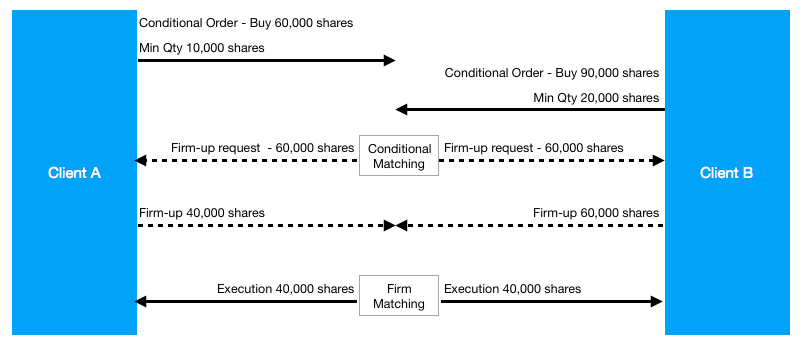
\includegraphics[width=\textwidth]{chapters/chapter_tech/figures/CondFlowChart2.png} 
	\caption{Conditional Order Matching Mechanism. \label{fig:CondFlowChart2}}
	\end{figure}

\item{\textbf{External Indication of Interest (IOIs):}} Certain pools, in an attempt to improve fill rates for dark orders, might broadcast IOIs to liquidity providers and other destinations. This practice is generally quite controversial as it raises questions about undesirable information leakage, and most participants would opt out of the functionality if at all possible.
\end{itemize}


These examples are not meant to be exhaustive, but nonetheless highlight the flexibility that exists for ATS compared to traditional exchanges and help explain their rise in popularity over time.